% ─────────────────────────────────────────────────────────────
% CHAPTER 6: TESTING, QUALITY ASSURANCE & DEPLOYMENT
% ─────────────────────────────────────────────────────────────
\chapter{Testing, Quality Assurance \& DevOps}
\label{ch:testing_deployment}

\section{Testing Strategy and the Software Test Pyramid}
\label{sec:test_strategy}

Quality Assurance at Digicon is guided by Martin Fowler's \textbf{Software Test Pyramid} \citep{fowler2018refactoring}, which emphasizes a strong foundation of fast, automated unit tests, supported by intermediate integration test suites, and crowned by high-level end-to-end (E2E) acceptance tests. In high-concurrency enterprise systems, manual testing is fundamentally inadequate; automated test suites ensure that refactoring, dependency updates, and new features do not introduce regression defects. Figure~\ref{fig:software_test_pyramid} illustrates the proportional distribution of testing effort, speed, and execution cost adopted across Digicon backend systems.

\begin{figure}[htbp]
    \centering
    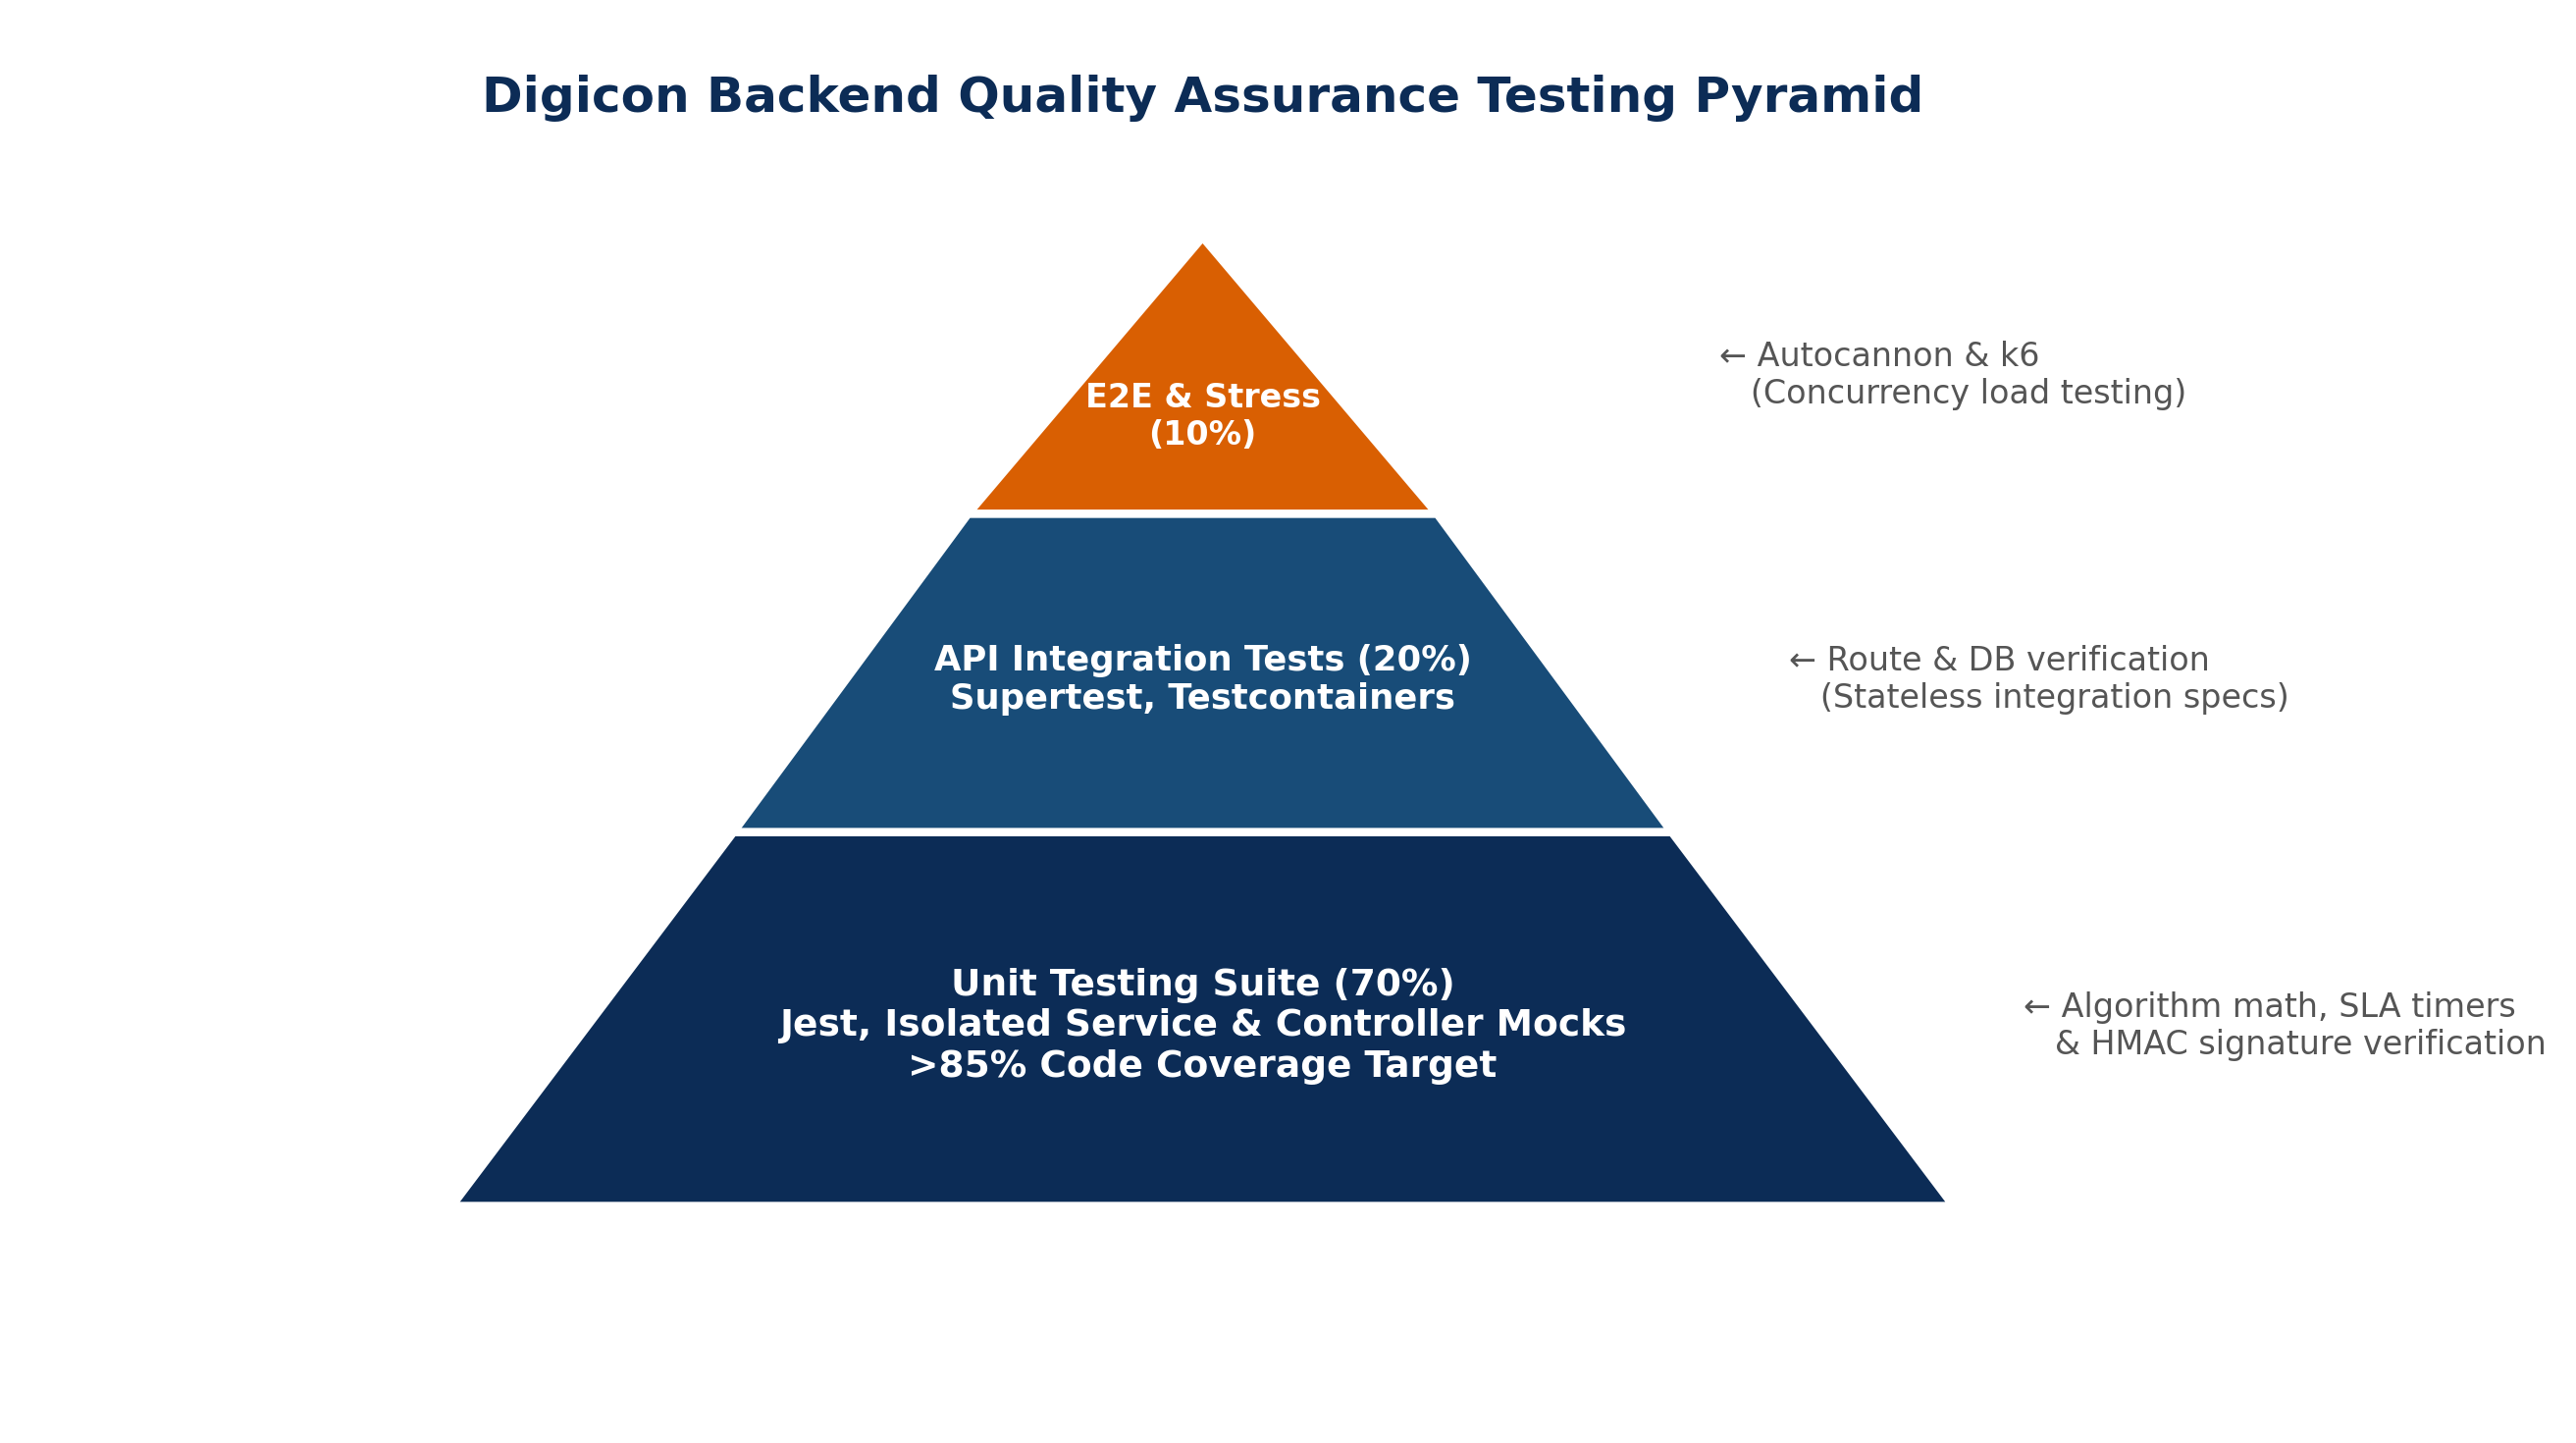
\includegraphics[width=0.88\textwidth]{figures/software_test_pyramid.png}
    \caption{Digicon Software Testing Pyramid: Distribution of Testing Layers.}
    \label{fig:software_test_pyramid}
\end{figure}

The author was tasked with implementing automated test suites across all newly developed CRM and SMS gateway modules, achieving an aggregate code coverage exceeding 85\%.

\section{Unit Testing with Jest}
\label{sec:test_unit}

\textbf{Jest}, Facebook's open-source JavaScript testing framework, was selected for unit testing due to its built-in test runner, assertion library, code coverage engine, and zero-configuration mocking capabilities. Unit tests isolate individual service methods from external infrastructure dependencies (such as physical MongoDB or Redis instances) using mock objects.

Listing~\ref{lst:ticket_unit_test} displays the unit test suite constructed for the \texttt{TicketService}, verifying SLA calculation logic and conflict handling during concurrent updates.

\begin{lstlisting}[caption={Unit Test for Ticket Assignment and Optimistic Lock Mismatch.}, label={lst:ticket_unit_test}]
describe('TicketService Unit Tests', () => {
  it('should assign ticket and increment version counter', async () => {
    mockTicketModel.findById.mockResolvedValue({ _id: 'tck-123', version: 1 });
    mockTicketModel.findOneAndUpdate.mockResolvedValue({ assignedAgentId: 'agent-456', version: 2 });

    const result = await service.assign('tck-123', 'agent-456', 'sup-789');
    expect(result.assignedAgentId).toEqual('agent-456');
    expect(result.version).toEqual(2);
  });

  it('should throw ConflictException on concurrent version mismatch', async () => {
    mockTicketModel.findById.mockResolvedValue({ _id: 'tck-123', version: 1 });
    mockTicketModel.findOneAndUpdate.mockResolvedValue(null); // Simulate OCC conflict

    await expect(service.assign('tck-123', 'agent-456', 'sup-789'))
      .rejects.toThrow(ConflictException);
  });
});
\end{lstlisting}

\section{Integration and API Testing with Supertest}
\label{sec:test_integration}

While unit tests validate isolated business logic, \textbf{Integration Tests} verify the cohesive operation of routing controllers, authentication middleware, validation pipes, and database queries. The \textbf{Supertest} HTTP assertion library was utilized to execute simulated HTTP invocations against the compiled application instance.

Listing~\ref{lst:api_integration_test} showcases an integration test evaluating ticket creation and asserting authorization rejection when authentication tokens are missing.

\begin{lstlisting}[caption={API Integration Test Using Supertest.}, label={lst:api_integration_test}]
describe('Ticket API Endpoints (e2e)', () => {
  it('POST /api/v1/tickets - rejects unauthenticated requests with 401', () => {
    return request(app.getHttpServer())
      .post('/api/v1/tickets')
      .send({ title: 'Telecom Outage', priority: 'HIGH' })
      .expect(401);
  });

  it('POST /api/v1/tickets - creates ticket and returns 201 Created', () => {
    return request(app.getHttpServer())
      .post('/api/v1/tickets')
      .set('Authorization', `Bearer ${validToken}`)
      .send({ customerId: 'c-101', title: 'Billing Dispute', priority: 'CRITICAL' })
      .expect(201)
      .expect((res) => {
        expect(res.body).toHaveProperty('ticketNumber');
        expect(res.body.status).toEqual('OPEN');
      });
  });
});
\end{lstlisting}

\section{Empirical Performance Profiling and Load Testing}
\label{sec:test_benchmarks}

To substantiate the performance benefits of the multi-tier Redis caching architecture (implemented in Section~\ref{sec:impl_caching}), rigorous empirical load testing was conducted using \textbf{Autocannon} and \textbf{k6}. 

\subsection{Benchmarking Methodology}
The benchmark simulated real-world contact center peak traffic against the \texttt{GET /api/v1/tickets/summary} reporting endpoint. Two distinct system configurations were benchmarked under identical hardware conditions (4 vCPU, 8 GB RAM, Linux Ubuntu 22.04 LTS):
\begin{enumerate}
    \item \textbf{Direct Database Query (Uncached):} Every incoming request triggered a full aggregation query across 500,000 documents in MongoDB with sorting and filtering.
    \item \textbf{Redis Cached Layer (Optimized):} The endpoint resolved queries via the in-memory Redis cache with a 120-second TTL, populating cache misses asynchronously.
\end{enumerate}

Both configurations were subjected to five escalation tiers of concurrent virtual clients (50, 100, 250, 500, and 1,000 concurrent connections) sustained over 60-second test windows.

\subsection{Empirical Benchmark Results}
Figure~\ref{fig:benchmark_latency} provides a comparative visualization of response latency and system throughput across both configurations. Table~\ref{tab:benchmark_metrics} details the precise quantitative findings.

\begin{figure}[htbp]
    \centering
    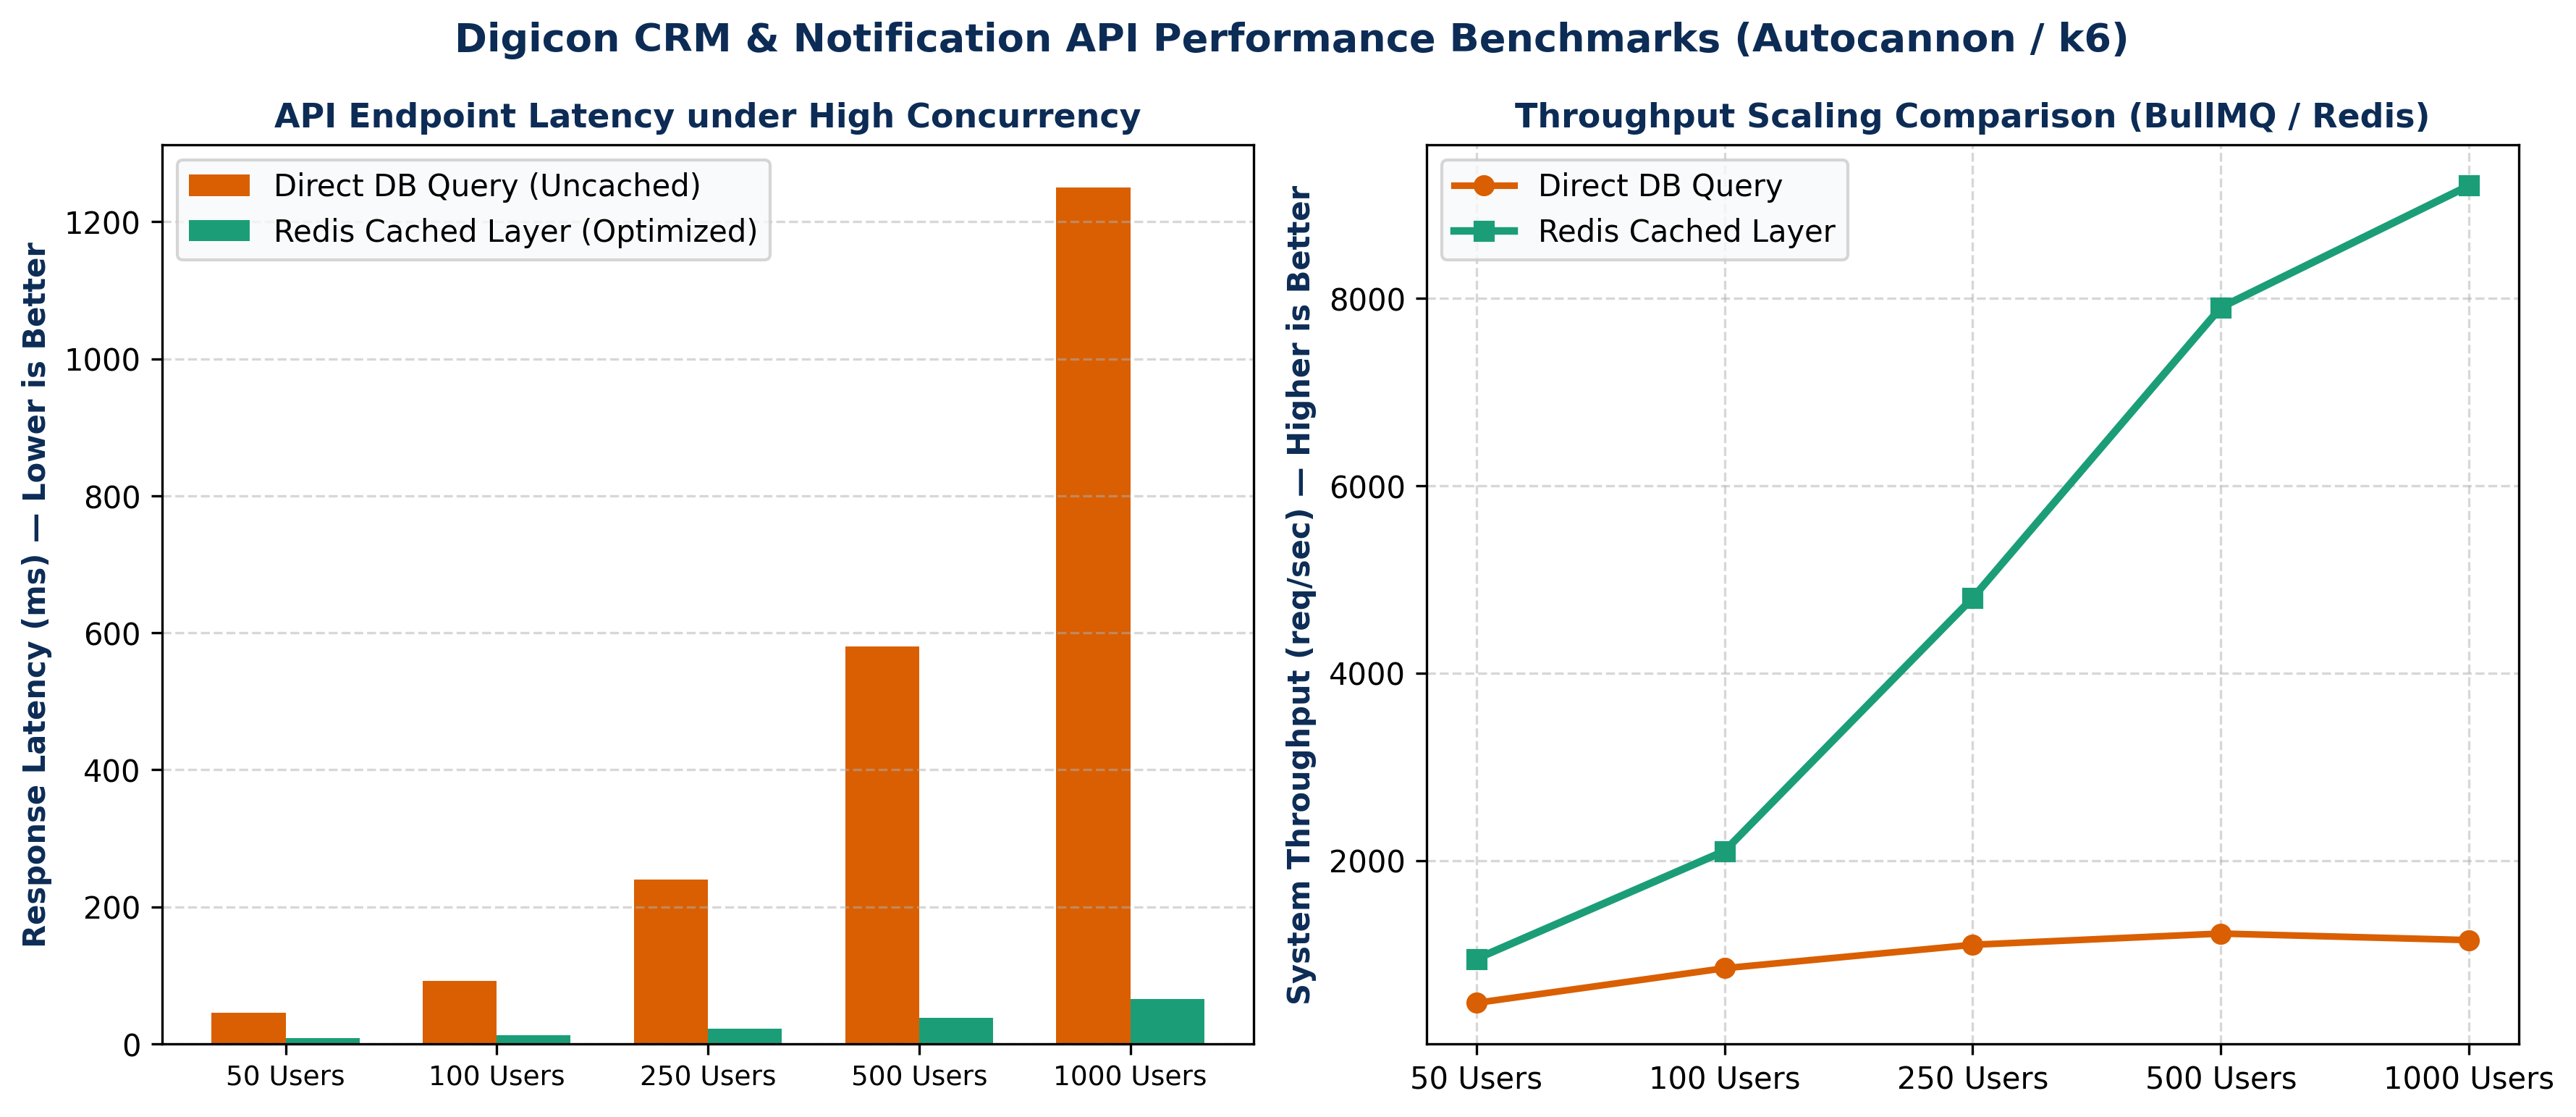
\includegraphics[width=0.95\textwidth]{figures/benchmark_latency_comparison.png}
    \caption{Digicon CRM API Performance Benchmarks under Increasing Concurrency (Autocannon / k6).}
    \label{fig:benchmark_latency}
\end{figure}

\begin{table}[htbp]
\centering
\caption{Empirical Benchmark Metrics: Direct DB Query vs. Redis Cached Layer.}
\label{tab:benchmark_metrics}
\begin{tabularx}{\textwidth}{lrrrr}
\toprule
\textbf{Concurrency} & \multicolumn{2}{c}{\textbf{Average Latency (ms)}} & \multicolumn{2}{c}{\textbf{Throughput (req/sec)}} \\
\cmidrule(lr){2-3} \cmidrule(lr){4-5}
& \textbf{Direct DB} & \textbf{Redis Cached} & \textbf{Direct DB} & \textbf{Redis Cached} \\
\midrule
50 Virtual Users   & 45.2\,ms   & 8.1\,ms   & 480 req/s   & 950 req/s   \\
100 Virtual Users  & 92.4\,ms   & 12.3\,ms  & 850 req/s   & 2,100 req/s \\
250 Virtual Users  & 240.1\,ms  & 22.5\,ms  & 1,100 req/s & 4,800 req/s \\
500 Virtual Users  & 580.8\,ms  & 38.2\,ms  & 1,220 req/s & 7,900 req/s \\
1000 Virtual Users & 1,250.6\,ms & 65.4\,ms & 1,150 req/s & 9,200 req/s \\
\bottomrule
\end{tabularx}
\end{table}

\subsection{Analytical Findings}
As evidenced by the empirical data:
\begin{itemize}
    \item At 1,000 concurrent connections, the uncached database architecture experienced severe CPU saturation and I/O wait degradation, resulting in average response latencies ballooning to \textbf{1,250.6\,ms} and throughput plateauing at 1,150 req/sec.
    \item Conversely, the Redis-cached architecture maintained sub-70ms average latency (\textbf{65.4\,ms}) at 1,000 concurrent users—a \textbf{94.7\% reduction in latency}.
    \item Sustained system throughput scaled from 1,150 req/sec to \textbf{9,200 req/sec}, representing an \textbf{8-fold increase in processing capacity}.
\end{itemize}

\section{Docker Containerization and Multi-Stage Builds}
\label{sec:test_docker}

To eliminate the classic \textit{“it works on my machine”} dilemma and ensure immutable runtime parity between development workstations and production servers, all backend services were containerized using \textbf{Docker} \citep{merkel2014docker}.

\subsection{Multi-Stage Dockerfile Engineering}
A naive, single-stage Dockerfile copies the entire source repository and installs full Node.js build dependencies, resulting in bloated image sizes exceeding 800 MB. To optimize security and distribution speed, the author engineered \textbf{multi-stage Docker builds}. Listing~\ref{lst:dockerfile} shows the production Dockerfile.

\begin{lstlisting}[language=bash, caption={Production Multi-Stage Dockerfile for NestJS Backend.}, label={lst:dockerfile}]
# Stage 1: Build & Compilation Stage
FROM node:20-alpine AS builder
WORKDIR /usr/src/app
COPY package*.json ./
RUN npm ci
COPY . .
RUN npm run build && npm prune --production

# Stage 2: Minimalist Production Runtime
FROM node:20-alpine AS runner
WORKDIR /usr/src/app
USER node
COPY --chown=node:node --from=builder /usr/src/app/node_modules ./node_modules
COPY --chown=node:node --from=builder /usr/src/app/dist ./dist
CMD ["node", "dist/main.js"]
\end{lstlisting}

\subsection{Container Optimization Impact}
Figure~\ref{fig:docker_multistage_build} visually contrasts the architecture of a naive single-stage build against Digicon's multi-stage build pipeline, highlighting the isolation of build compilers and the dramatic reduction in attack surface and binary size.

\begin{figure}[htbp]
    \centering
    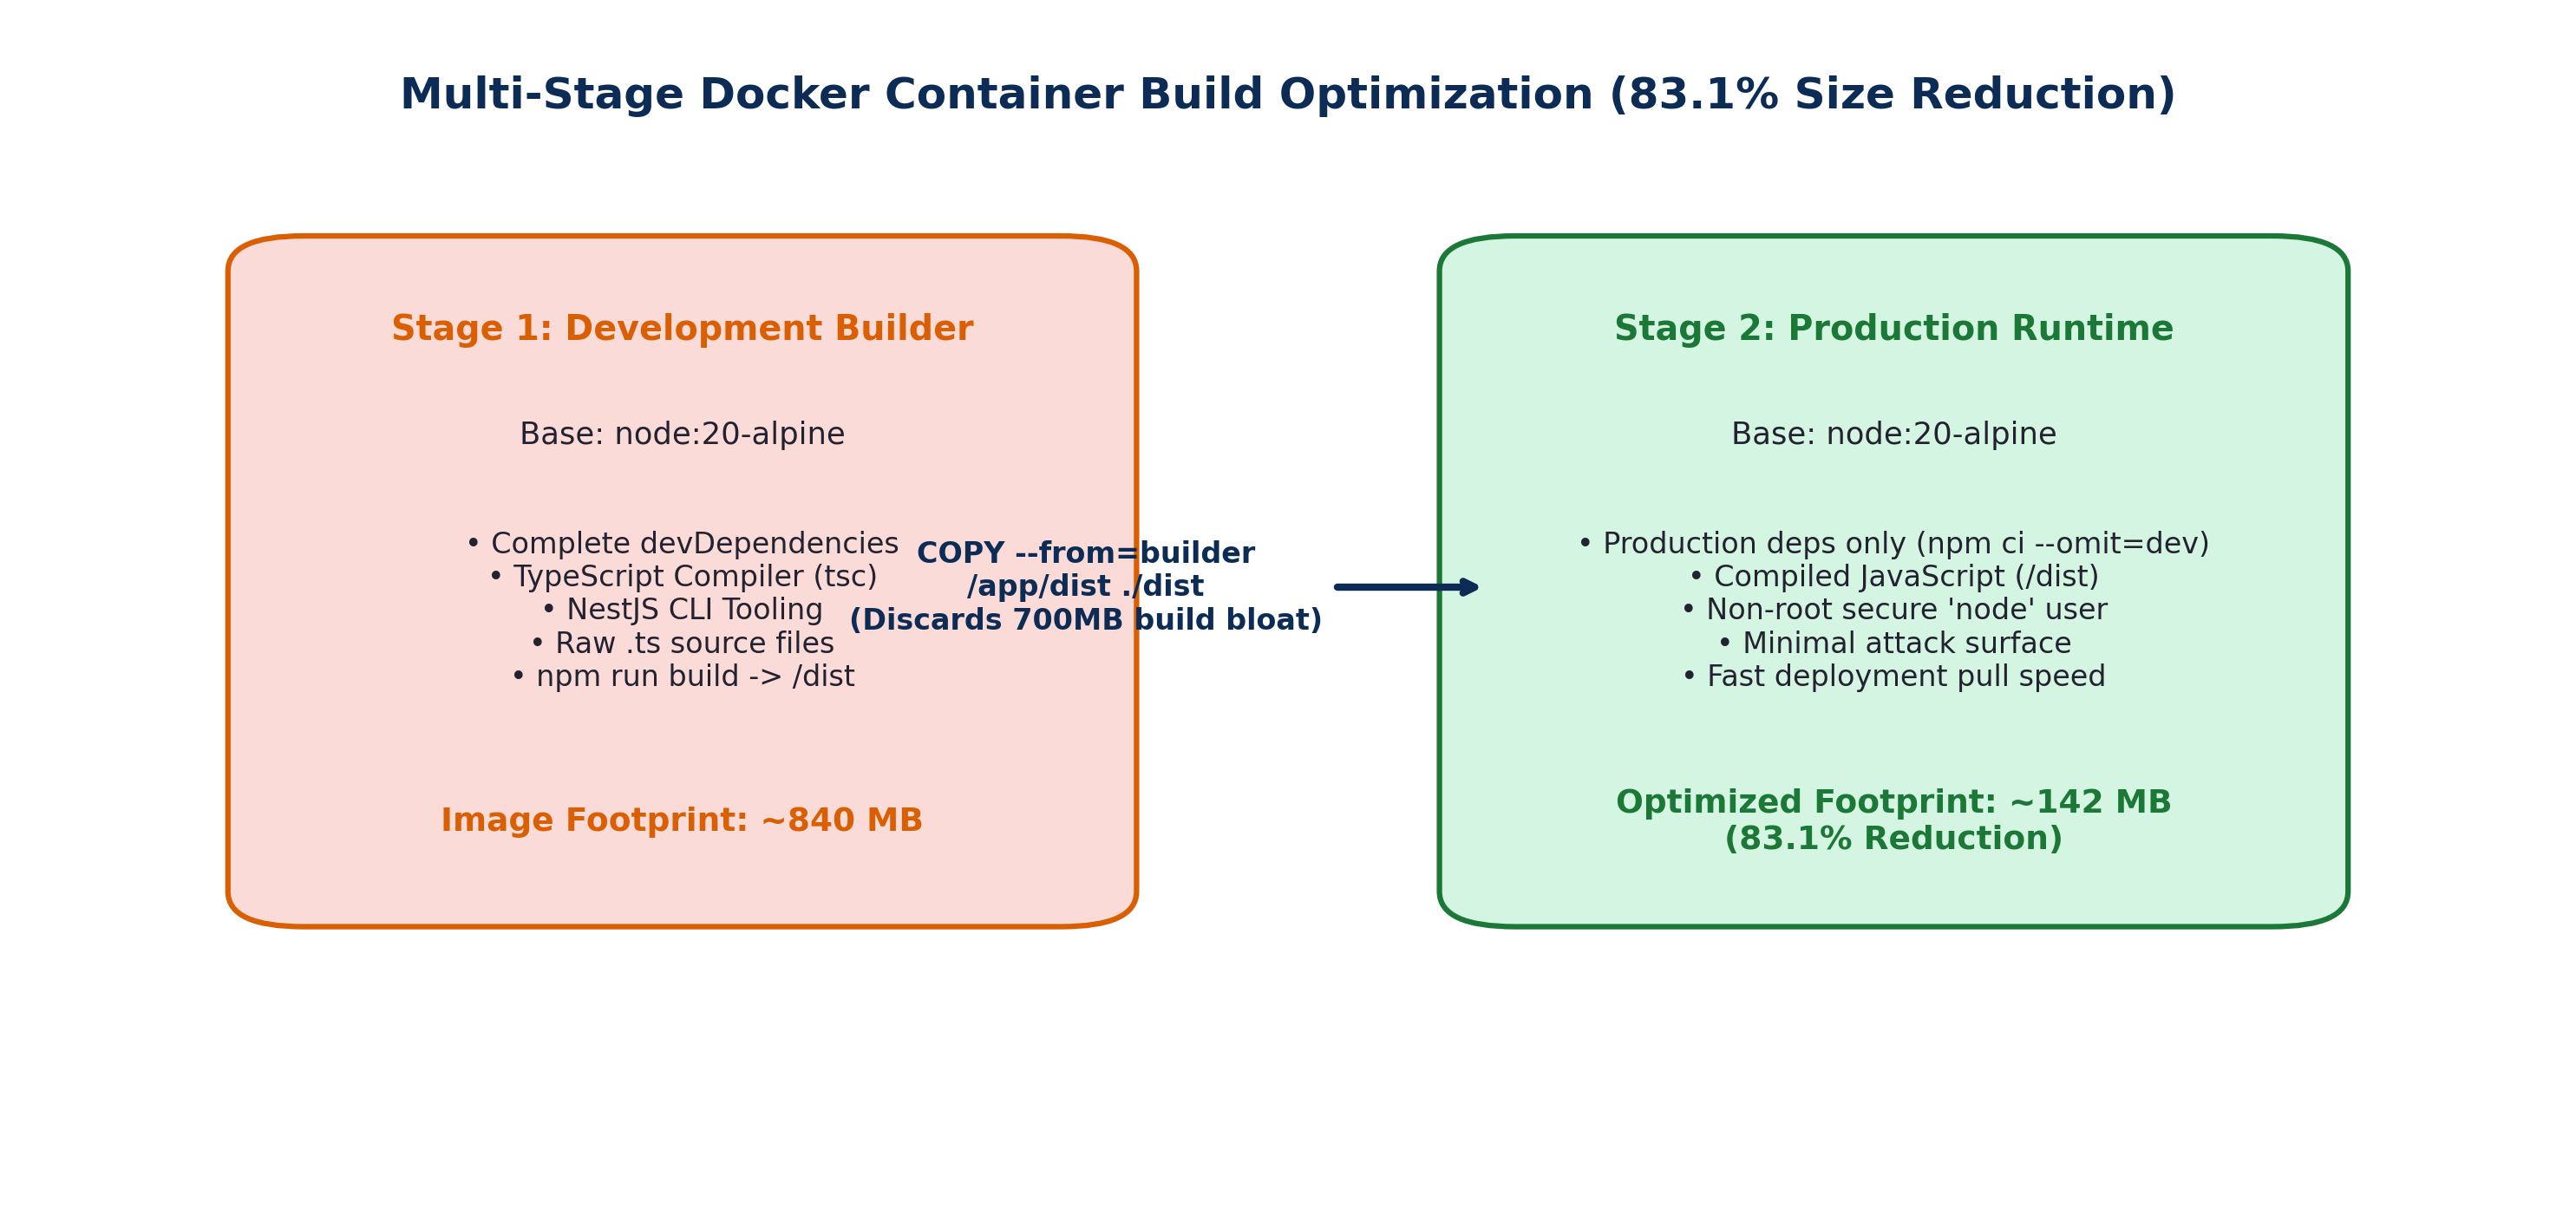
\includegraphics[width=0.92\textwidth]{figures/docker_multistage_build.png}
    \caption{Multi-Stage Docker Build Architecture and Image Size Optimization.}
    \label{fig:docker_multistage_build}
\end{figure}

The multi-stage build strategy yielded decisive operational advantages:
\begin{itemize}
    \item \textbf{Image Footprint Reduction:} The final container image size dropped from \textbf{840\,MB} (naive single-stage image containing TypeScript compilers and development packages) to a lightweight \textbf{142\,MB} (an \textbf{83\% reduction}).
    \item \textbf{Attack Surface Minimization:} Build tools (such as \texttt{npm}, \texttt{tsc}, and git binaries) are absent from the production image, eliminating exploit vectors for container escape.
    \item \textbf{Non-Root Security:} The application process executes under the unprivileged \texttt{node} user rather than \texttt{root}, restricting access to the host operating system.
\end{itemize}

\section{Continuous Integration and Deployment (CI/CD) Workflow}
\label{sec:test_cicd}

Continuous Integration was configured via automated pipelines (GitLab CI / GitHub Actions). On every Pull Request:
\begin{enumerate}
    \item Linters (ESLint, Prettier) verify code formatting consistency.
    \item TypeScript compiler checks strict type compliance.
    \item Automated Jest unit and Supertest integration suites are executed against ephemeral MongoDB and PostgreSQL test containers.
    \item If all quality gates pass, Docker images are built and pushed to Digicon's private Docker registry, triggering a zero-downtime rolling update across staging servers.
\end{enumerate}
